\documentclass[mathserif]{beamer}

\setbeamertemplate{frametitle}[default][center]%Centers the frame title.
\setbeamertemplate{navigation symbols}{}%Removes navigation symbols.
\setbeamertemplate{footline}{\raisebox{5pt}{\makebox[\paperwidth]{\hfill\makebox[10pt]{\scriptsize\insertframenumber}}}}
\setbeamertemplate{caption}[numbered]

\usepackage{amssymb,amsfonts,amsmath,latexsym,amsthm}
%\usepackage[usenames,dvipsnames]{color}
%\usepackage[]{graphicx}
%\usepackage[space]{grffile}
\usepackage{mathrsfs}   % fancy math font
% \usepackage[font=small,skip=0pt]{caption}
\usepackage[skip=0pt]{caption}
\usepackage{subcaption}
\usepackage{verbatim}
\usepackage{url}
\usepackage{bm}
\usepackage{dsfont}
\usepackage{extarrows}
\usepackage{multirow}
%\newcommand{\tth}   {\mbox{$\theta$}}
\newcommand{\thh}   {\mbox{$\theta$}}
\newcommand{\su}   {\mbox{$\sigma^2$}}
\newcommand{\so}   {\mbox{$\sigma_0^2$}}
\newcommand{\ko}   {\mbox{$\kappa_0$}}
\newcommand{\no}   {\mbox{$\nu_0$}}
\newcommand{\mo}   {\mbox{$\mu_0$}}
\newcommand{\ti}   {\mbox{$\tilde{x}$}}
\newcommand{\la}   {\mbox{$\lambda$}}
\newcommand{\bx}   {\mbox{$\bm{x}$}}
\newcommand{\bZ}   {\mbox{$\bm{Z}$}}
\newcommand{\bX}   {\mbox{$\bm{X}$}}
\newcommand{\bY}   {\mbox{$\bm{Y}$}}
\newcommand{\bA}   {\mbox{$\bm{A}$}}
\newcommand{\ba}   {\mbox{$\bm{a}$}}
\newcommand{\bb}   {\mbox{$\bm{b}$}}
\newcommand{\bt}   {\mbox{$\bm{t}$}}
\newcommand{\bz}   {\mbox{$\bm{z}$}}
\newcommand{\bw}   {\mbox{$\bm{w}$}}
\newcommand{\bbeta}   {\mbox{$\bm{\beta}$}}

\newcommand{\be}   {\mbox{$\bm{e}$}}
\newcommand{\bu}   {\mbox{$\bm{u}$}}
\newcommand{\bv}   {\mbox{$\bm{v}$}}
\newcommand{\sig}   {\mbox{$\Sigma$}}
\newcommand{\sigx}   {\mbox{$\Sigma_{XX}$}}
\newcommand{\sigxy}   {\mbox{$\Sigma_{XY}$}}
\newcommand{\tr}   {\mbox{$\text{tr}$}}
\newcommand{\ddet}   {\mbox{$\text{det}$}}
\newcommand\independent{\protect\mathpalette{\protect\independenT}{\perp}}
\def\independenT#1#2{\mathrel{\rlap{$#1#2$}\mkern2mu{#1#2}}}

\newcommand{\Expect}[1]{\ensuremath{\mathbf{E}\left[ #1 \right]}}
%\newcommand{\Var}[1]{\ensuremath{\mathrm{Var}\left[ #1 \right]}}
%\newcommand{\Cov}[1]{\ensuremath{\mathrm{Cov}\left[ #1 \right]}}
\newcommand{\MSE}{\ensuremath{\mathrm{MSE}}}
\newcommand{\RSS}{\ensuremath{\mathrm{RSS}}}
\newcommand{\Prob}[1]{\ensuremath{\mathrm{Pr}\left( #1 \right)}}
\newcommand{\ProbEst}[1]{\ensuremath{\widehat{\mathrm{Pr}}\left( #1 \right)}}
\DeclareMathOperator*{\argmin}{argmin} % thanks, wikipedia!
\DeclareMathOperator*{\argmax}{argmax} % thanks, wikipedia!
\DeclareMathOperator*{\sgn}{sgn} % thanks, wikipedia!

\newcommand{\lam}{\lambda}
\newcommand{\bmu}{\bm{\mu}}
%\newcommand{\bx}{\ensuremath{\mathbf{X}}}
\newcommand{\X}{\ensuremath{\mathbf{X}}}
\newcommand{\w}{\ensuremath{\mathbf{w}}}
\newcommand{\h}{\ensuremath{\mathbf{h}}}
\newcommand{\V}{\ensuremath{\mathbf{V}}}
%\newcommand{\tr}{\operatorname{tr}}

%\newcommand{\bx}{\ensuremath{\mathbf{X}}}
%\newcommand{\X}{\ensuremath{\mathbf{x}}}
%\newcommand{\w}{\ensuremath{\mathbf{w}}}
%\newcommand{\h}{\ensuremath{\mathbf{h}}}
%\newcommand{\V}{\ensuremath{\mathbf{v}}}
%\newcommand{\Cov}{\text{Cov}}
%\newcommand{\Var}{\text{Var}}

\DeclareMathOperator{\var}{Var}
\DeclareMathOperator{\cov}{Cov}
\newcommand{\Var}[1]{\ensuremath{\mathrm{Var}\left[ #1 \right]}}
\newcommand{\Cov}[1]{\ensuremath{\mathrm{Cov}\left[ #1 \right]}}


\newcommand{\indep}{\rotatebox{90}{\ensuremath{\models}}}
\newcommand{\notindep}{\not\hspace{-.05in}\indep}







\usepackage{float,bm}
\floatstyle{boxed}
\newfloat{code}{tp}{code}
\floatname{code}{Code Example}
%\newcommand{\tth}   {\mbox{$\theta$}}
\newcommand{\thh}   {\mbox{$\theta$}}
\newcommand{\su}   {\mbox{$\sigma^2$}}
\newcommand{\so}   {\mbox{$\sigma_0^2$}}
\newcommand{\ko}   {\mbox{$\kappa_0$}}
\newcommand{\no}   {\mbox{$\nu_0$}}
\newcommand{\mo}   {\mbox{$\mu_0$}}
\newcommand{\ti}   {\mbox{$\tilde{x}$}}
\newcommand{\la}   {\mbox{$\lambda$}}
\newcommand{\bx}   {\mbox{$\bm{x}$}}
\newcommand{\bZ}   {\mbox{$\bm{Z}$}}
\newcommand{\bX}   {\mbox{$\bm{X}$}}
\newcommand{\bY}   {\mbox{$\bm{Y}$}}
\newcommand{\bA}   {\mbox{$\bm{A}$}}
\newcommand{\ba}   {\mbox{$\bm{a}$}}
\newcommand{\bb}   {\mbox{$\bm{b}$}}
\newcommand{\bt}   {\mbox{$\bm{t}$}}
\newcommand{\bz}   {\mbox{$\bm{z}$}}
\newcommand{\bw}   {\mbox{$\bm{w}$}}
\newcommand{\bbeta}   {\mbox{$\bm{\beta}$}}

\newcommand{\be}   {\mbox{$\bm{e}$}}
\newcommand{\bu}   {\mbox{$\bm{u}$}}
\newcommand{\bv}   {\mbox{$\bm{v}$}}
\newcommand{\sig}   {\mbox{$\Sigma$}}
\newcommand{\sigx}   {\mbox{$\Sigma_{XX}$}}
\newcommand{\sigxy}   {\mbox{$\Sigma_{XY}$}}
\newcommand{\tr}   {\mbox{$\text{tr}$}}
\newcommand{\ddet}   {\mbox{$\text{det}$}}
\newcommand\independent{\protect\mathpalette{\protect\independenT}{\perp}}
\def\independenT#1#2{\mathrel{\rlap{$#1#2$}\mkern2mu{#1#2}}}

\newcommand{\Expect}[1]{\ensuremath{\mathbf{E}\left[ #1 \right]}}
%\newcommand{\Var}[1]{\ensuremath{\mathrm{Var}\left[ #1 \right]}}
%\newcommand{\Cov}[1]{\ensuremath{\mathrm{Cov}\left[ #1 \right]}}
\newcommand{\MSE}{\ensuremath{\mathrm{MSE}}}
\newcommand{\RSS}{\ensuremath{\mathrm{RSS}}}
\newcommand{\Prob}[1]{\ensuremath{\mathrm{Pr}\left( #1 \right)}}
\newcommand{\ProbEst}[1]{\ensuremath{\widehat{\mathrm{Pr}}\left( #1 \right)}}
\DeclareMathOperator*{\argmin}{argmin} % thanks, wikipedia!
\DeclareMathOperator*{\argmax}{argmax} % thanks, wikipedia!
\DeclareMathOperator*{\sgn}{sgn} % thanks, wikipedia!

\newcommand{\lam}{\lambda}
\newcommand{\bmu}{\bm{\mu}}
%\newcommand{\bx}{\ensuremath{\mathbf{X}}}
\newcommand{\X}{\ensuremath{\mathbf{X}}}
\newcommand{\w}{\ensuremath{\mathbf{w}}}
\newcommand{\h}{\ensuremath{\mathbf{h}}}
\newcommand{\V}{\ensuremath{\mathbf{V}}}
%\newcommand{\tr}{\operatorname{tr}}

%\newcommand{\bx}{\ensuremath{\mathbf{X}}}
%\newcommand{\X}{\ensuremath{\mathbf{x}}}
%\newcommand{\w}{\ensuremath{\mathbf{w}}}
%\newcommand{\h}{\ensuremath{\mathbf{h}}}
%\newcommand{\V}{\ensuremath{\mathbf{v}}}
%\newcommand{\Cov}{\text{Cov}}
%\newcommand{\Var}{\text{Var}}

\DeclareMathOperator{\var}{Var}
\DeclareMathOperator{\cov}{Cov}
\newcommand{\Var}[1]{\ensuremath{\mathrm{Var}\left[ #1 \right]}}
\newcommand{\Cov}[1]{\ensuremath{\mathrm{Cov}\left[ #1 \right]}}


\newcommand{\indep}{\rotatebox{90}{\ensuremath{\models}}}
\newcommand{\notindep}{\not\hspace{-.05in}\indep}






%\usepackage{fontspec}
%\setmainfont{Tahoma}

%\newcommand{\lam}{\lambda}
%\newcommand{\bmu}{\bm{\mu}}
%%\newcommand{\bx}{\ensuremath{\mathbf{X}}}
%\newcommand{\X}{\ensuremath{\mathbf{x}}}
%\newcommand{\w}{\ensuremath{\mathbf{w}}}
%\newcommand{\h}{\ensuremath{\mathbf{h}}}
%\newcommand{\V}{\ensuremath{\mathbf{v}}}
%\newcommand{\cov}{\text{Cov}}
%\newcommand{\var{\text{Var}}}

%\DeclareMathOperator{\var}{Var}
%\DeclareMathOperator{\cov}{Cov}

%\newcommand{\indep}{\rotatebox{90}{\ensuremath{\models}}}
%\newcommand{\notindep}{\not\hspace{-.05in}\indep}

\usepackage{graphicx} %The mode "LaTeX => PDF" allows the following formats: .jpg  .png  .pdf  .mps
\graphicspath{{./PresentationPictures/}} %Where the figures folder is located
\usepackage{listings}
\usepackage{media9}
\usepackage{movie15}
\addmediapath{./Movies/}

\newcommand{\beginbackup}{
   \newcounter{framenumbervorappendix}
   \setcounter{framenumbervorappendix}{\value{framenumber}}
}
\newcommand{\backupend}{
   \addtocounter{framenumbervorappendix}{-\value{framenumber}}
   \addtocounter{framenumber}{\value{framenumbervorappendix}} 
}


%\usepackage{algorithm2e}
\usepackage[ruled,lined]{algorithm2e}
\def\algorithmautorefname{Algorithm}
\SetKwIF{If}{ElseIf}{Else}{if}{then}{else if}{else}{endif}
%\usepackage{times}
%\usepackage[tbtags]{amsmath}
%\usepackage{amssymb}
\usepackage{amsfonts}
%\usepackage{slfortheorems}
\usepackage{epsfig}
\usepackage{graphicx}
%\usepackage[small]{caption}
%\usepackage[square]{natbib}
%\newcommand{\newblock}{}
%\bibpunct{(}{)}{;}{a}{}{,}
%\bibliographystyle{ims}
%\usepackage[letterpaper]{geometry}
%\usepackage{color}
%\setlength{\parindent}{0pt}

\usepackage{natbib}
\bibpunct{(}{)}{;}{a}{}{,}
%\usepackage{hyperref}

\DeclareMathOperator*{\Exp}{Exp}
\DeclareMathOperator*{\TExp}{TExp}
\DeclareMathOperator*{\Bernoulli}{Bernoulli}
\DeclareMathOperator*{\Beta}{Beta}
\DeclareMathOperator*{\Ga}{Gamma}
\DeclareMathOperator*{\TGamma}{TGamma}
\DeclareMathOperator*{\Poisson}{Poisson}
\DeclareMathOperator*{\Binomial}{Binomial}
\DeclareMathOperator*{\NormalGamma}{NormalGamma}
\DeclareMathOperator*{\InvGamma}{InvGamma}
\DeclareMathOperator*{\Cauchy}{Cauchy}
\DeclareMathOperator*{\Uniform}{Uniform}
\DeclareMathOperator*{\Gumbel}{Gumbel}
\DeclareMathOperator*{\Pareto}{Pareto}
\DeclareMathOperator*{\Mono}{Mono}
\DeclareMathOperator*{\Geometric}{Geometric}
\DeclareMathOperator*{\Wishart}{Wishart}

\newcommand{\N}{\mathcal{N}}

\newcommand{\R}{\mathbb{R}}
\newcommand{\Z}{\mathbb{Z}}
\newcommand{\E}{\mathbb{E}}
\renewcommand{\Pr}{\mathbb{P}}
\newcommand{\I}{\mathds{1}}
\newcommand{\V}{\mathbb{V}}

% Math operators
\DeclareMathOperator*{\diag}{diag}
\DeclareMathOperator*{\median}{median}
\DeclareMathOperator*{\Vol}{Vol}

% Miscellaneous commands
\newcommand{\iid}{\stackrel{\mathrm{iid}}{\sim}}
\newcommand{\matrixsmall}[1]{\bigl(\begin{smallmatrix}#1\end{smallmatrix} \bigr)}

\newcommand{\items}[1]{\begin{itemize} #1 \end{itemize}}

\newcommand{\todo}[1]{\emph{\textcolor{red}{(#1)}}}

\newcommand{\branch}[4]{
\left\{
	\begin{array}{ll}
		#1  & \mbox{if } #2 \\
		#3 & \mbox{if } #4
	\end{array}
\right.
}

% approximately proportional to
\def\app#1#2{%
  \mathrel{%
    \setbox0=\hbox{$#1\sim$}%
    \setbox2=\hbox{%
      \rlap{\hbox{$#1\propto$}}%
      \lower1.3\ht0\box0%
    }%
    \raise0.25\ht2\box2%
  }%
}
\def\approxprop{\mathpalette\app\relax}

\newcommand{\btheta}{{\bm\theta}}
\newcommand{\bbtheta}{{\pmb{\bm\theta}}}

%\usepackage{zref-savepos}
%
%\newcounter{restofframe}
%\newsavebox{\restofframebox}
%\newlength{\mylowermargin}
%\setlength{\mylowermargin}{2pt}
%
%\newenvironment{restofframe}{%
%    \par%\centering
%    \stepcounter{restofframe}%
%    \zsavepos{restofframe-\arabic{restofframe}-begin}%
%    \begin{lrbox}{\restofframebox}%
%}{%
%    \end{lrbox}%
%    \setkeys{Gin}{keepaspectratio}%
%    \raisebox{\dimexpr-\height+\ht\strutbox\relax}[0pt][0pt]{%
%    \resizebox*{!}{\dimexpr\zposy{restofframe-\arabic{restofframe}-begin}sp-\zposy{restofframe-\arabic{restofframe}-end}sp-\mylowermargin\relax}%
%        {\usebox{\restofframebox}}%
%    }%
%    \vskip0pt plus 1filll\relax
%    \mbox{\zsavepos{restofframe-\arabic{restofframe}-end}}%
%    \par
%}


\usepackage{tikz}
\usetikzlibrary{arrows}

%\usepackage[usenames,dvipsnames]{xcolor}
\usepackage{tkz-berge}
\usetikzlibrary{fit,shapes}

\usepackage{calc}
%%
%% The tikz package is used for doing the actual drawing.
%\usepackage{tikz}
%%
%% In order to be able to put arrowheads in the middle of directed edges, we need an extra library.
\usetikzlibrary{decorations.markings}
%%
%% The next line says how the "vertex" style of nodes should look: drawn as small circles.
\tikzstyle{vertex}=[circle, draw, inner sep=0pt, minimum size=6pt]
%%
%% Next, we make a \vertex command as a shorthand in place of \node[vertex} to get that style.
\newcommand{\vertex}{\node[vertex]}
%%
%% Finally, we declare a "counter", which is what LaTeX calls an integer variable, for use in
%% the calculations of angles for evenly spacing vertices in circular arrangements.
\newcounter{Angle}

\newtheoremstyle{example}
{\topsep} % space above
{\topsep} % space below
{} % body font
{} % indent
{\bf} % head font
{:} % punctuation between head and body
{0.5em} % space after head
{} % manually specify head
%{\thmname{#1}\thmnumber{ #2}\thmnote{:#3}} % manually specify head

\theoremstyle{example}
\newtheorem{ex}{Example}[section]

\newtheoremstyle{definition}
{\topsep} % space above
{\topsep} % space below
{} % body font
{} % indent
{\sc} % head font
{:} % punctuation between head and body
{0.5em} % space after head
{} % manually specify head
%{\thmname{#1}\thmnumber{ #2}\thmnote{:#3}} % manually specify head

\theoremstyle{definition}
\newtheorem{defn}{Definition}[section]

\theoremstyle{rem}
\newtheorem{rem}{Remark}[section]

\newtheoremstyle{theorem}
{\topsep} % space above
{\topsep} % space below
{} % body font
{} % indent
{\sc} % head font
{:} % punctuation between head and body
{0.5em} % space after head
{} % manually specify head
%{\thmname{#1}\thmnumber{ #2}\thmnote{:#3}} % manually specify head

\theoremstyle{theorm}
\newtheorem{thm}{Theorem}[section]



%%%to add in new counter for slides in beamer

%\setbeamertemplate{footline}{
%  \leavevmode%
%  \hbox{%
%  \begin{beamercolorbox}[wd=.333333\paperwidth,ht=2.25ex,dp=1ex,center]{author in head/foot}%
%    \usebeamerfont{author in head/foot}\insertshortauthor~~(\insertshortinstitute)
%  \end{beamercolorbox}%
%  \begin{beamercolorbox}[wd=.333333\paperwidth,ht=2.25ex,dp=1ex,center]{title in head/foot}%
%    \usebeamerfont{title in head/foot}\insertshorttitle
%  \end{beamercolorbox}%
%  \begin{beamercolorbox}[wd=.333333\paperwidth,ht=2.25ex,dp=1ex,right]{date in head/foot}%
%    \usebeamerfont{date in head/foot}\insertshortdate{}\hspace*{2em}
%    \insertframenumber{} \hspace*{2ex} % hier hat's sich ge�ndert
%  \end{beamercolorbox}}%
%  \vskip0pt%
%}



%%%%%

\newcommand*\oldmacro{}
\let\oldmacro\insertshortauthor
\renewcommand*\insertshortauthor{
  \leftskip=.3cm
\insertframenumber\,/\,\inserttotalframenumber\hfill\oldmacro}




%\excludecomment{notbeamer}
%\includecomment{beamer}



\title{Intro to Markov Chain Monte Carlo}
\author{Rebecca C. Steorts \\ Bayesian Methods and Modern Statistics: STA 360/601}
\date{Module 7 }

\begin{document}

\maketitle

%\frame{
%\frametitle{Announcements}
%\begin{enumerate}
%\item Modules will be compartmentalized into each class. 
%\item All questions will be held until the last 10--15 minutes of class. 
%\item If you have a question in lecture, write it down. 
%\item If you think there is a typo, write it down. 
%\item I will cold call on students in class, to make sure that students are understanding and understanding the material.
%\item If you are being rude to me or to another student, you will be asked to leave the class.
%\item We will talk about the grading policy for final grades more after midterm 2. 
%\item Extra problems to work for the exam: there are a long list of suggested exercises in each module. Exercises in Baby Bayes. In fact, one of these was partially on the exam! 
%\end{enumerate}
%
%
%
%}



\frame{
\frametitle{Gibbs sampling} 

Instead of moving into the Metropolis algorithm, we now move into
Gibbs sampling, which is a special case of it. 

\vskip 1em

We will return back to the Metropolis algorithm later and go through the actual algorithm
and implementation in detail! 




}



\frame{
\frametitle{Two-stage Gibbs sampler}
\begin{itemize}
\item Suppose $p(x,y)$ is a p.d.f.\ or p.m.f.\ that is difficult to sample from directly.  
\item Suppose, though, that we \textit{can} easily sample from the conditional distributions $p(x|y)$ and $p(y|x)$. 
\item  The Gibbs sampler proceeds as follows: 
\begin{enumerate}
\item set $x$ and $y$ to some initial starting values
\item then sample $x|y$, then sample $y|x$,\\ then $x|y$, and so on.
\end{enumerate}
\end{itemize}

}


\frame{
\frametitle{Two-stage Gibbs sampler}
\begin{enumerate}
\item[0.] Set \textcolor{blue}{$(x_0,y_0)$} to some starting value.
\item[1.] Sample $x_1\sim p(x|y_0)$, that is, from the conditional distribution $X\mid Y=y_0$. \\
\textcolor{blue}{Current state: $(x_1, y_0)$}\\
          Sample $y_1\sim p(y|x_1)$, that is, from the conditional distribution $Y\mid X=x_1$.\\
    \textcolor{blue}{      Current state: $(x_1, y_1)$}\\
\item[2.] Sample $x_2\sim p(x|y_1)$, that is, from the conditional distribution $X\mid Y=y_1$. \\
    \textcolor{blue}{      Current state: $(x_2, y_1)$}\\
          Sample $y_2\sim p(y|x_2)$, that is, from the conditional distribution $Y\mid X=x_2$. \\
            \textcolor{blue}{      Current state: $(x_2, y_2)$}\\
        $\vdots$
\end{enumerate}
Repeat iterations 1 and 2, M times. 

This procedure defines a sequence of pairs of random variables
$$ (X_0,Y_0), (X_1,Y_1), (X_2,Y_2), (X_3,Y_3), \ldots$$

}

\frame{
\frametitle{Markov chain and dependence}


$$ (X_0,Y_0), (X_1,Y_1), (X_2,Y_2), (X_3,Y_3), \ldots$$ satisfies the property of being a Markov chain. 

\vskip 1em

The conditional distribution of $(X_i,Y_i)$ given all of the previous pairs depends only on $(X_{i-1},Y_{i-1})$

\vskip 1em

$(X_0,Y_0), (X_1,Y_1), (X_2,Y_2), (X_3,Y_3), \ldots$ are not iid samples (Think about why). 

}

\frame{
\frametitle{Ideal Properties of MCMC}

\begin{itemize}
\item $(x_0,y_0)$ chosen to be in a region of high probability under $p(x,y)$, but often this
is not so easy. 
%\item Instead, we run the chain for a long time. 
\item We run the chain for M iterations and discard the first $B$ samples $(X_1,Y_1),\ldots,(X_B,Y_B)$. This is called \emph{burn-in}.
% future: We will discuss how to choose $B$ in ???
%\item When using a burn-in period, the choice of starting point it is not particularly
%important---a poor choice will simply require a longer burn-in period.
\item Typically: if you run the chain long enough, the choice of $B$ doesn't matter. 

\item Roughly speaking, the performance of an MCMC algorithm---that is, how quickly the sample averages $\frac{1}{N}\sum_{i = 1}^N h(X_i,Y_i)$
converge---is referred to as the \emph{mixing rate}. 
\item An algorithm with good performance is said to ``have good mixing'', or ``mix well''.

\end{itemize}


}

\frame{
\frametitle{Toy Example}

Suppose we want to sample from the bivariate distribution:
$$p(x,y) \propto e^{-x y}\I(x,y\in (0, c))$$
where $c>0$, and $(0,c)$ denotes the (open) interval between $0$ and $c$. 
(This example is due to Casella \& George, 1992.)
}

\frame{
\frametitle{Toy Example}
\begin{itemize}
\item The Gibbs sampling approach is to alternately sample from $p(x|y)$ and $p(y|x)$.  
\item Note $p(x,y)$ is
symmetric with respect to $x$ and $y$.
\item Hence, only need to derive one of these and then we can get the other one by just swapping $x$ and $y$.
\item Let's look at $p(x|y).$
\end{itemize}
}

\frame{
\frametitle{Toy Example}
$$p(x,y) \propto e^{-x y}\I(x,y\in (0, c))$$

$$p(x|y) \underset{x}{\propto} p(x,y) \underset{x}{\propto} e^{-x y}\I(0<x<c)\underset{x}{\propto} \Exp(x|y)\I(x<c).\footnote{Under $\propto$, we write the random variable ($x$) for clarity.}
$$\begin{itemize}
\item $p(x|y)$ is a \emph{truncated} version of the $\Exp(y)$ distribution
\item It is the same as taking $X\sim\Exp(y)$ and
 conditioning on it being less than $c$, i.e., $X\mid X<c$.
\item Let's refer to this as the $\TExp(y,(0,c))$ distribution.
\end{itemize}
}

\frame{
\frametitle{Toy Example}
An easy way to generate a sample from $Z\sim\TExp(\theta,(0,c))$, is:
\begin{enumerate}
    \item Sample $U\sim \Uniform(0,F(c|\theta))$ where $$F(x|\theta) = 1-e^{-\theta x}$$ is the $\Exp(\theta)$ c.d.f.
    \item Set $Z = F^{-1}(U|\theta)$ where $$F^{-1}(u|\theta) = -(1/\theta)\log(1 - u)$$ is the inverse c.d.f.\ for $u\in(0,1)$.
\end{enumerate}
%To verify the last step: apply the rejection principle (along with the inverse cdf technique). 
%Do this on your own.
Verify the last step on your own.

}


\frame{

Let's apply Gibbs sampling, denoting $S=(0,c)$.
\begin{enumerate}
    \item[0.] Initialize $x_0,y_0\in S$.
    \item[1.] Sample $x_1\sim \TExp(y_0,S)$, then sample $y_1\sim \TExp(x_1,S).$
    \item[2.] Sample $x_2\sim \TExp(y_1,S)$, then sample $y_2\sim \TExp(x_2,S).$\\
        $\vdots$
    \item[$N$.] Sample $x_N\sim \TExp(y_{N-1},S)$, sample $y_N\sim \TExp(x_N,S).$
\end{enumerate}
Figure \ref{figure:toy} demonstrates the algorithm, with $c = 2$ and initial point $(x_0, y_0) = (1, 1)$.

}

\frame{

\begin{figure}
  \begin{center}
    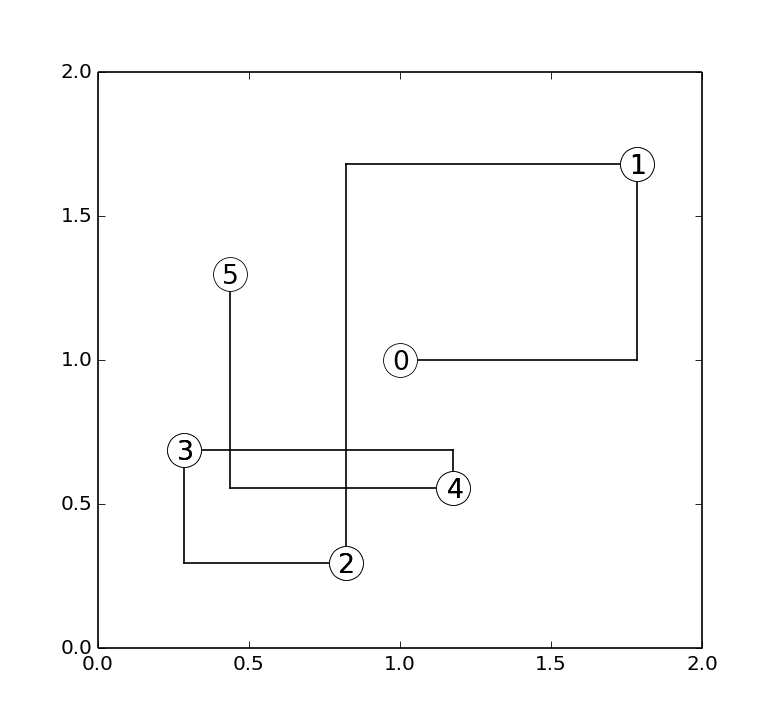
\includegraphics[width=0.48\textwidth]{examples/toy-numbered.png}
    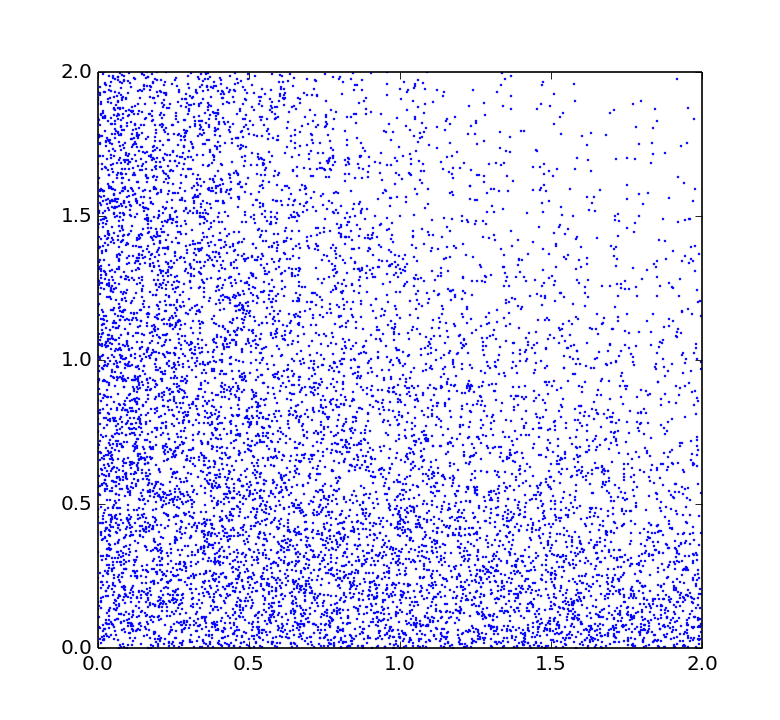
\includegraphics[width=0.48\textwidth]{examples/toy-scatter.png}
  \end{center}
  \caption{(Left) Schematic representation of the first 5 Gibbs sampling iterations/sweeps/scans. (Right) Scatterplot of samples from $10^4$ Gibbs sampling iterations.}
  \label{figure:toy}
\end{figure}



}

\frame{
\frametitle{Example: Normal with semi-conjugate prior}

Consider
$X_1,\ldots,X_n|\mu,\lambda\,\iid \N(\mu,\lambda^{-1})$.
Then independently consider
\begin{align*}
& \bm\mu \sim \N(\mu_0,\lambda_0^{-1})\\
& \bm\lambda \sim \Ga(a,b)
\end{align*}

This is called a semi-conjugate situation, in the sense that the prior on $\mu$ is conjugate for each fixed value of $\lambda$, and the prior on $\lambda$ is conjugate for each fixed value of $\mu$.

\vskip 1em

For ease of notation, denote the observed data points by $x_{1:n}.$

}

\frame{


We know that for the Normal--Normal model, we know that for any fixed value of $\lambda$,
$$\bm\mu|\lambda,x_{1:n}\, \sim \,\N(M_\lambda,L_\lambda^{-1})$$
 where $$L_\lambda =\lambda_0+ n\lambda \;\;  \text{and} \;\;
 M_\lambda =\frac{\lambda_0\mu_0+\lambda\sum_{i = 1}^n x_i}{\lambda_0+ n\lambda}.$$
\pause
For any fixed value of $\mu$, it is straightforward to derive\footnote{do this on your own} that
\begin{align}\label{equation:lambda-semi-conjugate}
\bm\lambda|\mu, x_{1:n}\,\sim\,\Ga(A_\mu, B_\mu)
\end{align}
where $A_\mu = a + n/2$ and
$$ B_\mu = b +\tfrac{1}{2}\textstyle\sum (x_i -\mu)^2 = n\hat\sigma^2 + n (\bar x-\mu)^2$$
where $\hat\sigma^2 = \frac{1}{n}\sum (x_i -\bar x)^2$. 




}

\frame{

To implement Gibbs sampling in this example, each iteration consists of sampling:
\begin{align*}
    & \bm\mu|\lambda,x_{1:n}\, \sim \,\N(M_\lambda,L_\lambda^{-1})\\
    & \bm\lambda|\mu, x_{1:n}\,\sim\,\Ga(A_\mu, B_\mu).
\end{align*}


}

\frame{
\frametitle{Pareto example}

Distributions of sizes and frequencies often tend to follow a ``power law'' distribution. 
\begin{itemize}
    \item wealth of individuals
    \item size of oil reserves
    \item size of cities
    \item word frequency
    \item returns on stocks
\end{itemize}
}
\frame{
\frametitle{Power Law Distribution}
The Pareto distribution with shape $\alpha>0$ and scale $c >0$ has p.d.f.\
$$ \Pareto(x|\alpha,c) = \frac{\alpha c^\alpha}{x^{\alpha+1}}\I(x>c)\propto \frac{1}{x^{\alpha+1}}\I(x>c).$$
This is referred to as a power law distribution, because the p.d.f.\ is proportional to $x$ raised to a power.
Notice that $c$ is a lower bound on the observed values.
In this example, we'll see how Gibbs sampling can be used to perform inference for $\alpha$ and $c$. 


}

\frame{

\begin{table}
\small
\centering
\begin{tabular}{clr}
Rank & City & Population \\
\hline
1  &  Charlotte   &  731424 \\
2  &  Raleigh   &  403892 \\
3  &  Greensboro   &  269666 \\
4  &  Durham   &  228330 \\
5  &  Winston-Salem   &  229618 \\
6  &  Fayetteville   &  200564 \\
7  &  Cary  &  135234 \\
8  &  Wilmington   &  106476 \\
9  &  High Point  &  104371 \\
10  &  Greenville   &  84554 \\
11  &  Asheville   &  85712 \\
12  &  Concord   &  79066 \\
\vdots  &  \vdots   &  \vdots \\
44  &  Havelock  &  20735 \\
45  &  Carrboro  &  19582 \\
46  &  Shelby   &  20323 \\
47  &  Clemmons  &  18627 \\
48  &  Lexington   &  18931 \\
49  &  Elizabeth City   &  18683 \\
50  &  Boone   &  17122 \\
\hline
\end{tabular}
\vspace{1em}
\caption{Populations of the 50 largest cities in the state of North Carolina, USA.}
\label{table:cities}
\end{table}



}

\frame{
\frametitle{Parameter Interpretations}

\begin{itemize}
\item $\alpha$ tells us the scaling relationship between the size of cities and their probability of occurring. 
\begin{itemize}
\item Let $\alpha = 1$. 
\item 
Density looks like $1/x^{\alpha +1} = 1/x^2$.
\item Cities with 10,000--20,000 inhabitants occur roughly $10^{\alpha+1} = 100$
    times as frequently as cities with 100,000--110,000 inhabitants.
%    (or $10^{\alpha +1}/10 = 10$ times as frequently as cities with
%    100,000--200,000 inhabitants).
\end{itemize}
\item $c$ represents the cutoff point---any cities smaller than this were not included in the dataset.
\end{itemize}
}


\frame{
To keep things as simple as possible, let's use an (improper) default prior:
$$p(\alpha,c) \propto \I(\alpha,c>0).$$

\vskip 1em
Recall from Module 4:
\begin{itemize}
\item An \emph{improper/default prior} is a nonnegative function of the parameters which integrates to infinity.
\item  Often (but not always!)\ the resulting ``posterior'' will be proper.
\item It is important that the ``posterior'' be proper, since otherwise the whole Bayesian framework breaks down.
\end{itemize}



}

\frame{
Recall
\textcolor{blue}{
\begin{align}
p(x|\alpha,c) &= \frac{\alpha c^\alpha}{x^{\alpha+1}}\I(x>c)\\
&\I(\alpha,c>0)
\end{align}
}
Let's derive the posterior:
\begin{align}
    p(\alpha,c|x_{1:n}) & \overset{\text{def}}{\underset{\alpha,c}{\propto}} p(x_{1:n}|\alpha,c)p(\alpha,c)\notag\\ 
    &\underset{\alpha,c}{\propto}\I(\alpha,c>0)\prod_{i=1}^n \frac{\alpha c^\alpha}{x_i^{\alpha+1}}\I(x_i>c) \notag\\
    & = \frac{\alpha^n c^{n\alpha}}{(\prod x_i)^{\alpha+1}} \I(c<x_*)\I(\alpha,c>0)\label{equation:Pareto-posterior}
                        % & = \alpha^n \Big(\prod_{i=1}^n c/x_i\Big)^\alpha \I(c<x_*)
\end{align}
where $x_* = \min\{x_1,\ldots,x_n\}$. 
\vskip 1em
As a joint distribution on $(\alpha,c)$, 
\begin{itemize}
\item this does not seem to have a recognizable form, 
\item and it is not clear how we might sample from it directly.
\end{itemize}
}

\frame{
Let's try Gibbs sampling! 
\vskip 1emTo use Gibbs, we need to be able to sample $\alpha|c,x_{1:n}$ and $c|\alpha,x_{1:n}$. 
\vskip 1em
By Equation \ref{equation:Pareto-posterior}, we find that
\begin{align*}
p(\alpha|c,x_{1:n})&\underset{\alpha}{\propto}p(\alpha,c|x_{1:n})
\underset{\alpha}{\propto} \frac{\alpha^n c^{n\alpha}}{(\prod x_i)^\alpha}\I(\alpha>0) \\
&= \alpha^n\exp\big(-\alpha(\textstyle\sum\log x_i - n\log c)\big)\I(\alpha>0) \\
&\underset{\alpha}{\propto} \Ga\big(\alpha\,\big\vert\, n+1,\,\textstyle\sum\log x_i - n\log c\big),
\end{align*}
and
\begin{align*}
p(c|\alpha, x_{1:n})\underset{c}{\propto}p(\alpha,c|x_{1:n})
\underset{c}{\propto} c^{n\alpha}\I(0<c<x_*),
\end{align*}
which we will define to be Mono$(\alpha, x_*)$


}

\frame{
\frametitle{Defining the Mono distribution}
For $a>0$ and $b>0$, define the distribution $\Mono(a,b)$ (for monomial) with p.d.f.
$$ \Mono(x|a,b)\propto x^{a-1}\I(0<x<b). $$
Since $\int_0^b x^{a -1}d x = b^a/a$, we have
$$ \Mono(x|a,b) =\frac{a}{b^a}x^{a-1}\I(0<x<b), $$
and for $0<x<b$, the c.d.f.\ is
$$ F(x|a,b) =\int_0^x \Mono(y|a,b)d y = \frac{a}{b^a}\frac{x^a}{a} = \frac{x^a}{b^a}. $$
}

\frame{
To use the inverse c.d.f.\ technique, we solve for the inverse of $F$ on $0<x<b$:
Let $u = \frac{x^a}{b^a}$ and solve for $x.$
\begin{align}
u &= \frac{x^a}{b^a} \\
b^a u &= x^a \\ 
b u^{1/a} &= x 
\end{align}
Can sample from $\Mono(a,b)$ by drawing $U\sim \Uniform(0,1)$ and setting $X=b U^{1/a}$.\footnote{ It turns out that this is an inverse of the Pareto distribution, in the sense that if $X\sim\Pareto(\alpha,c)$ then $1/X\sim\Mono(\alpha,1/c)$. }



}

\frame{
So, in order to use the Gibbs sampling algorithm to sample from the posterior $p(\alpha,c|x_{1:n})$, we initialize $\alpha$ and $c$, and then alternately update them by sampling:
\begin{align*}
\alpha|c,x_{1:n} \,&\sim\, \Ga\big(n+1,\,\textstyle\sum\log x_i - n\log c\big) \\
c|\alpha,x_{1:n}\,&\sim\, \Mono(n\alpha+1,\,x_*).
\end{align*}
}

\frame{
\frametitle{Ways of visualizing results}
 \textbf{Traceplots}. A traceplot simply shows the sequence of samples, for instance $\alpha_1,\ldots,\alpha_N$, or $c_1,\ldots, c_N$. Traceplots are a simple but very useful way to visualize how the sampler is behaving. 
 }

\frame{
\begin{figure}[htbp]
\begin{center}
 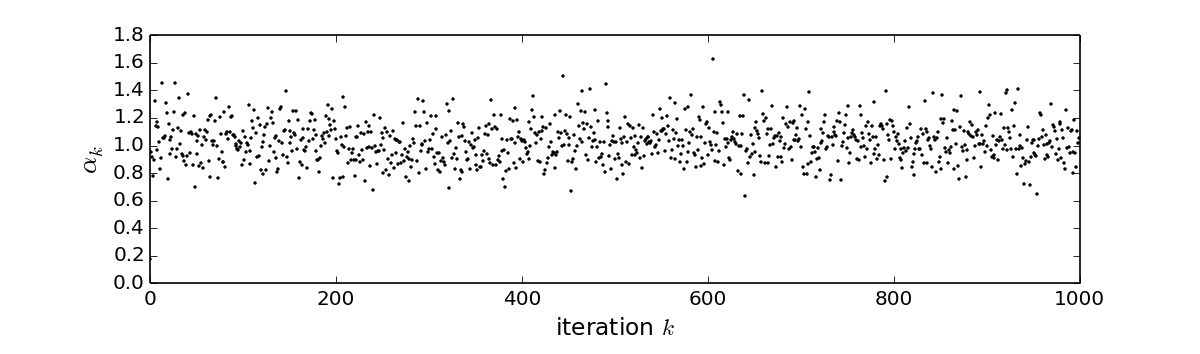
\includegraphics[width=0.65\textwidth]{examples/Pareto-a_trace.png}
\caption{Traceplot of $\alpha$}
\label{default}
\end{center}
\end{figure}


\begin{figure}[htbp]
\begin{center}
 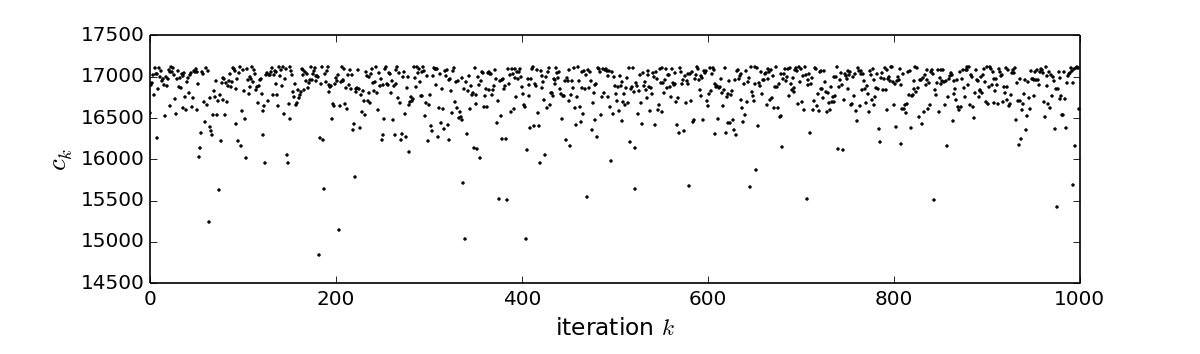
\includegraphics[width=0.65\textwidth]{examples/Pareto-c_trace.png}
\caption{Traceplot of c.}
\label{default}
\end{center}
\end{figure}

}

%\frame{
%
% \textbf{Scatterplot}. 
% \vskip 1em
% Scatterplot visualizes the estimated posterior distribution $p(\alpha, c|x_{1:n})$.
%  \vskip 1em
%  How can we also visualize the estimated posterior? plot(density())
%   \vskip 1em
% Boone is the smallest city, with a population of 17,122. 
%  \vskip 1em
% Posterior on $c$ is quite concentrated just under 17,122, which makes sense since $c$ represents the cutoff point in the sampling process.
%
%
%}

%\frame{
%\begin{figure}[htbp]
%\begin{center}
%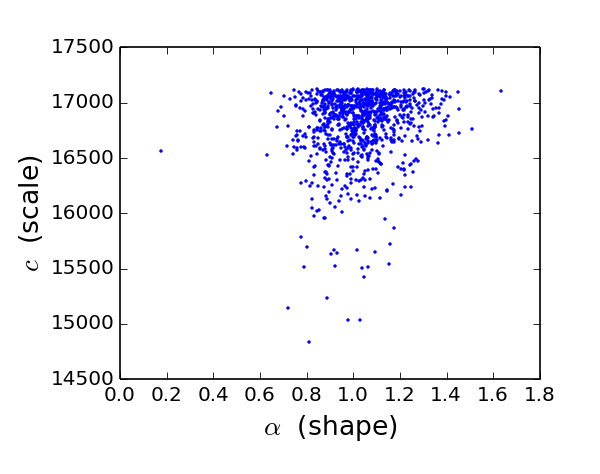
\includegraphics[width=0.8\textwidth]{examples/Pareto-scatterplot.png}
%\caption{Scatterplot of samples}
%\label{default}
%\end{center}
%\end{figure}
%}



\frame{
 \textbf{Estimated density}. We are primarily interested in the posterior on $\alpha$, since it tells us the scaling relationship between the size of cities and their probability of occurring. 
 
   \vskip 1em
 By making a histogram of the samples $\alpha_1,\ldots,\alpha_N$, we can estimate the posterior density $p(\alpha|x_{1:n})$. 
 
    \vskip 1em
 The two vertical lines indicate the lower $\ell$ and upper $u$ boundaries of an (approximate) 90\% credible interval $[\ell,u]$---that is, an interval that contains 90\% of the posterior probability:
$$\Pr\big(\bm\alpha\in [\ell, u] \big\vert x_{1:n}\big) = 0.9. $$
%The interval shown here is approximate since it's based on the samples. 
%This can be computed from the samples by sorting them $\alpha_{(1)}\leq \cdots\leq\alpha_{(N)}$ and setting
%$$\ell = \alpha_{(\lfloor 0.05 N\rfloor)}  \qquad u = \alpha_{(\lceil 0.95 N\rceil)} $$
%where $\lfloor x\rfloor$ and $\lceil x\rceil$ are the floor and ceiling functions, respectively.





}


\frame{
\begin{figure}[htbp]
\begin{center}
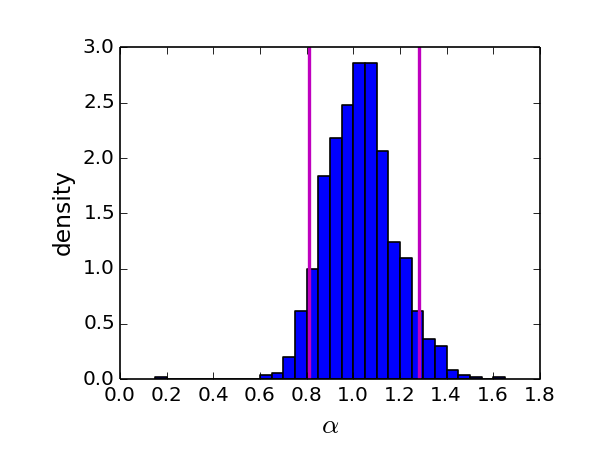
\includegraphics[width=0.9\textwidth]{examples/Pareto-a_density.png}\caption{Estimated density of $\alpha|x_{1:n}$ with $\approx$ 90 percent credible intervals.}
\label{default}
\end{center}
\end{figure}

}

\frame{
 \textbf{Running averages}. Panel (d) shows the running average $\frac{1}{k}\sum_{i = 1}^k\alpha_i$ for $k = 1,\ldots,N$.
    \vskip 1em
  In addition to traceplots, running averages such as this are a useful heuristic for visually assessing the convergence of the Markov chain. 
     \vskip 1em
  The running average shown in this example still seems to be meandering about a bit, suggesting that the sampler needs to be run longer (but this would depend on the level of accuracy desired).


}

\frame{
\begin{figure}[htbp]
\begin{center}
 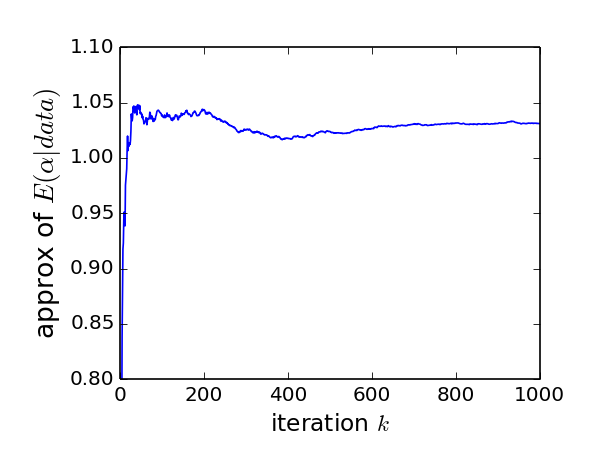
\includegraphics[width=0.8\textwidth]{examples/Pareto-a_means.png}
 \caption{Running average plot}
 \label{default}
\end{center}
\end{figure}

}

\frame{
\frametitle{Survival function}
A survival function is defined to be $$S(x) = \Pr(X>x) = 1-\Pr(X\leq x).$$
\vskip 1em


 Power law distributions are often displayed by plotting their survival function $S(x),$ on a log-log plot. 
 \vskip 1em
 Why?
  $S(x) = (c/x)^\alpha$ for the $\Pareto(\alpha,c)$ distribution and on a log-log plot this appears as a line with slope $-\alpha$.
 \vskip 1em
  The posterior survival function (or more precisely, the posterior predictive survival function), is $S(x|x_{1:n}) = \Pr(X_{n+1}>x\mid x_{1:n})$. 
  }
  
  \frame{
  Figure \ref{figure:Pareto}(e) shows an empirical estimate of the survival function (based on the empirical c.d.f., $\hat F(x) = \frac{1}{n}\sum_{i = 1}^n \I(x\geq x_i)$) along with the posterior survival function, approximated by
\begin{align}
S(x|x_{1:n}) &= \Pr(X_{n+1}>x\mid x_{1:n}) \\
&= \int \Pr(X_{n+1}>x\mid \alpha,c) p(\alpha,c|x_{1:n})d\alpha d c\\
&\approx\frac{1}{N}\sum_{i = 1}^N \Pr(X_{n+1}>x\mid \alpha_i,c_i)
=\frac{1}{N}\sum_{i = 1}^N (c_i/x)^{\alpha_i}.
\end{align}
This is computed for each $x$ in a grid of values.
\vskip 1em
[Think about why each line is true on your own].
}




\frame{
\begin{figure}[htbp]
\begin{center}
 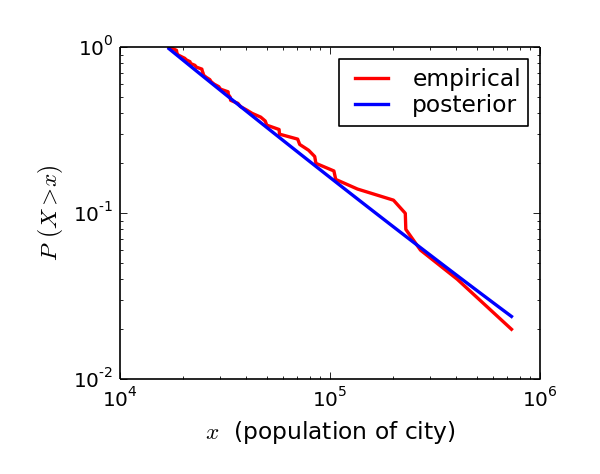
\includegraphics[width=0.8\textwidth]{examples/Pareto-survival-function.png}
 \caption{Empirical vs posterior survival function}
 \label{figure:Pareto}
\end{center}
\end{figure}

How could we get a better empirical approximation?

}



\end{document}